% Options for packages loaded elsewhere
\PassOptionsToPackage{unicode}{hyperref}
\PassOptionsToPackage{hyphens}{url}
\documentclass[
]{article}
\usepackage{xcolor}
\usepackage[margin=1in]{geometry}
\usepackage{amsmath,amssymb}
\setcounter{secnumdepth}{-\maxdimen} % remove section numbering
\usepackage{iftex}
\ifPDFTeX
  \usepackage[T1]{fontenc}
  \usepackage[utf8]{inputenc}
  \usepackage{textcomp} % provide euro and other symbols
\else % if luatex or xetex
  \usepackage{unicode-math} % this also loads fontspec
  \defaultfontfeatures{Scale=MatchLowercase}
  \defaultfontfeatures[\rmfamily]{Ligatures=TeX,Scale=1}
\fi
\usepackage{lmodern}
\ifPDFTeX\else
  % xetex/luatex font selection
\fi
% Use upquote if available, for straight quotes in verbatim environments
\IfFileExists{upquote.sty}{\usepackage{upquote}}{}
\IfFileExists{microtype.sty}{% use microtype if available
  \usepackage[]{microtype}
  \UseMicrotypeSet[protrusion]{basicmath} % disable protrusion for tt fonts
}{}
\makeatletter
\@ifundefined{KOMAClassName}{% if non-KOMA class
  \IfFileExists{parskip.sty}{%
    \usepackage{parskip}
  }{% else
    \setlength{\parindent}{0pt}
    \setlength{\parskip}{6pt plus 2pt minus 1pt}}
}{% if KOMA class
  \KOMAoptions{parskip=half}}
\makeatother
\usepackage{color}
\usepackage{fancyvrb}
\newcommand{\VerbBar}{|}
\newcommand{\VERB}{\Verb[commandchars=\\\{\}]}
\DefineVerbatimEnvironment{Highlighting}{Verbatim}{commandchars=\\\{\}}
% Add ',fontsize=\small' for more characters per line
\usepackage{framed}
\definecolor{shadecolor}{RGB}{248,248,248}
\newenvironment{Shaded}{\begin{snugshade}}{\end{snugshade}}
\newcommand{\AlertTok}[1]{\textcolor[rgb]{0.94,0.16,0.16}{#1}}
\newcommand{\AnnotationTok}[1]{\textcolor[rgb]{0.56,0.35,0.01}{\textbf{\textit{#1}}}}
\newcommand{\AttributeTok}[1]{\textcolor[rgb]{0.13,0.29,0.53}{#1}}
\newcommand{\BaseNTok}[1]{\textcolor[rgb]{0.00,0.00,0.81}{#1}}
\newcommand{\BuiltInTok}[1]{#1}
\newcommand{\CharTok}[1]{\textcolor[rgb]{0.31,0.60,0.02}{#1}}
\newcommand{\CommentTok}[1]{\textcolor[rgb]{0.56,0.35,0.01}{\textit{#1}}}
\newcommand{\CommentVarTok}[1]{\textcolor[rgb]{0.56,0.35,0.01}{\textbf{\textit{#1}}}}
\newcommand{\ConstantTok}[1]{\textcolor[rgb]{0.56,0.35,0.01}{#1}}
\newcommand{\ControlFlowTok}[1]{\textcolor[rgb]{0.13,0.29,0.53}{\textbf{#1}}}
\newcommand{\DataTypeTok}[1]{\textcolor[rgb]{0.13,0.29,0.53}{#1}}
\newcommand{\DecValTok}[1]{\textcolor[rgb]{0.00,0.00,0.81}{#1}}
\newcommand{\DocumentationTok}[1]{\textcolor[rgb]{0.56,0.35,0.01}{\textbf{\textit{#1}}}}
\newcommand{\ErrorTok}[1]{\textcolor[rgb]{0.64,0.00,0.00}{\textbf{#1}}}
\newcommand{\ExtensionTok}[1]{#1}
\newcommand{\FloatTok}[1]{\textcolor[rgb]{0.00,0.00,0.81}{#1}}
\newcommand{\FunctionTok}[1]{\textcolor[rgb]{0.13,0.29,0.53}{\textbf{#1}}}
\newcommand{\ImportTok}[1]{#1}
\newcommand{\InformationTok}[1]{\textcolor[rgb]{0.56,0.35,0.01}{\textbf{\textit{#1}}}}
\newcommand{\KeywordTok}[1]{\textcolor[rgb]{0.13,0.29,0.53}{\textbf{#1}}}
\newcommand{\NormalTok}[1]{#1}
\newcommand{\OperatorTok}[1]{\textcolor[rgb]{0.81,0.36,0.00}{\textbf{#1}}}
\newcommand{\OtherTok}[1]{\textcolor[rgb]{0.56,0.35,0.01}{#1}}
\newcommand{\PreprocessorTok}[1]{\textcolor[rgb]{0.56,0.35,0.01}{\textit{#1}}}
\newcommand{\RegionMarkerTok}[1]{#1}
\newcommand{\SpecialCharTok}[1]{\textcolor[rgb]{0.81,0.36,0.00}{\textbf{#1}}}
\newcommand{\SpecialStringTok}[1]{\textcolor[rgb]{0.31,0.60,0.02}{#1}}
\newcommand{\StringTok}[1]{\textcolor[rgb]{0.31,0.60,0.02}{#1}}
\newcommand{\VariableTok}[1]{\textcolor[rgb]{0.00,0.00,0.00}{#1}}
\newcommand{\VerbatimStringTok}[1]{\textcolor[rgb]{0.31,0.60,0.02}{#1}}
\newcommand{\WarningTok}[1]{\textcolor[rgb]{0.56,0.35,0.01}{\textbf{\textit{#1}}}}
\usepackage{graphicx}
\makeatletter
\newsavebox\pandoc@box
\newcommand*\pandocbounded[1]{% scales image to fit in text height/width
  \sbox\pandoc@box{#1}%
  \Gscale@div\@tempa{\textheight}{\dimexpr\ht\pandoc@box+\dp\pandoc@box\relax}%
  \Gscale@div\@tempb{\linewidth}{\wd\pandoc@box}%
  \ifdim\@tempb\p@<\@tempa\p@\let\@tempa\@tempb\fi% select the smaller of both
  \ifdim\@tempa\p@<\p@\scalebox{\@tempa}{\usebox\pandoc@box}%
  \else\usebox{\pandoc@box}%
  \fi%
}
% Set default figure placement to htbp
\def\fps@figure{htbp}
\makeatother
\setlength{\emergencystretch}{3em} % prevent overfull lines
\providecommand{\tightlist}{%
  \setlength{\itemsep}{0pt}\setlength{\parskip}{0pt}}
\usepackage{lscape}
\usepackage{booktabs}
\usepackage{longtable}
\usepackage{array}
\usepackage{multirow}
\usepackage{wrapfig}
\usepackage{float}
\usepackage{colortbl}
\usepackage{pdflscape}
\usepackage{tabu}
\usepackage{threeparttable}
\usepackage{threeparttablex}
\usepackage[normalem]{ulem}
\usepackage{makecell}
\usepackage{xcolor}
\usepackage{bookmark}
\IfFileExists{xurl.sty}{\usepackage{xurl}}{} % add URL line breaks if available
\urlstyle{same}
\hypersetup{
  pdftitle={Title Placeholder},
  hidelinks,
  pdfcreator={LaTeX via pandoc}}

\title{Title Placeholder}
\author{}
\date{\vspace{-2.5em}}

\begin{document}
\maketitle

\subsubsection{Load in Specific
Packages}\label{load-in-specific-packages}

\begin{Shaded}
\begin{Highlighting}[]
\FunctionTok{library}\NormalTok{(readr)}
\FunctionTok{library}\NormalTok{(tidyr)}
\FunctionTok{library}\NormalTok{(dplyr)}
\end{Highlighting}
\end{Shaded}

\begin{verbatim}
## 
## Attaching package: 'dplyr'
\end{verbatim}

\begin{verbatim}
## The following objects are masked from 'package:stats':
## 
##     filter, lag
\end{verbatim}

\begin{verbatim}
## The following objects are masked from 'package:base':
## 
##     intersect, setdiff, setequal, union
\end{verbatim}

\begin{Shaded}
\begin{Highlighting}[]
\FunctionTok{library}\NormalTok{(here)}
\end{Highlighting}
\end{Shaded}

\begin{verbatim}
## here() starts at C:/Users/romin/ToyRepo
\end{verbatim}

\begin{Shaded}
\begin{Highlighting}[]
\FunctionTok{library}\NormalTok{(lemon)}
\end{Highlighting}
\end{Shaded}

\begin{verbatim}
## Warning: package 'lemon' was built under R version 4.4.2
\end{verbatim}

\begin{Shaded}
\begin{Highlighting}[]
\FunctionTok{library}\NormalTok{(kableExtra)}
\end{Highlighting}
\end{Shaded}

\begin{verbatim}
## Warning: package 'kableExtra' was built under R version 4.4.2
\end{verbatim}

\begin{verbatim}
## 
## Attaching package: 'kableExtra'
\end{verbatim}

\begin{verbatim}
## The following object is masked from 'package:dplyr':
## 
##     group_rows
\end{verbatim}

\begin{Shaded}
\begin{Highlighting}[]
\FunctionTok{library}\NormalTok{(ggplot2)}
\end{Highlighting}
\end{Shaded}

\begin{verbatim}
## Warning: package 'ggplot2' was built under R version 4.4.2
\end{verbatim}

\begin{Shaded}
\begin{Highlighting}[]
\FunctionTok{library}\NormalTok{(}\FunctionTok{reshape}\NormalTok{())}
\end{Highlighting}
\end{Shaded}

\begin{verbatim}
## Warning: package 'reshape' was built under R version 4.4.2
\end{verbatim}

\begin{verbatim}
## 
## Attaching package: 'reshape'
\end{verbatim}

\begin{verbatim}
## The following object is masked from 'package:dplyr':
## 
##     rename
\end{verbatim}

\begin{verbatim}
## The following objects are masked from 'package:tidyr':
## 
##     expand, smiths
\end{verbatim}

\begin{Shaded}
\begin{Highlighting}[]
\FunctionTok{library}\NormalTok{(hexbin)}
\end{Highlighting}
\end{Shaded}

\begin{verbatim}
## Warning: package 'hexbin' was built under R version 4.4.2
\end{verbatim}

\begin{Shaded}
\begin{Highlighting}[]
\FunctionTok{library}\NormalTok{(data.table)}
\end{Highlighting}
\end{Shaded}

\begin{verbatim}
## 
## Attaching package: 'data.table'
\end{verbatim}

\begin{verbatim}
## The following object is masked from 'package:reshape':
## 
##     melt
\end{verbatim}

\begin{verbatim}
## The following objects are masked from 'package:dplyr':
## 
##     between, first, last
\end{verbatim}

\begin{Shaded}
\begin{Highlighting}[]
\FunctionTok{library}\NormalTok{(GGally)}
\end{Highlighting}
\end{Shaded}

\begin{verbatim}
## Warning: package 'GGally' was built under R version 4.4.2
\end{verbatim}

\begin{verbatim}
## Registered S3 method overwritten by 'GGally':
##   method from   
##   +.gg   ggplot2
\end{verbatim}

\begin{Shaded}
\begin{Highlighting}[]
\FunctionTok{library}\NormalTok{(formattable)}
\end{Highlighting}
\end{Shaded}

\begin{verbatim}
## Warning: package 'formattable' was built under R version 4.4.2
\end{verbatim}

\begin{Shaded}
\begin{Highlighting}[]
\FunctionTok{library}\NormalTok{(viridis)}
\end{Highlighting}
\end{Shaded}

\begin{verbatim}
## Warning: package 'viridis' was built under R version 4.4.2
\end{verbatim}

\begin{verbatim}
## Loading required package: viridisLite
\end{verbatim}

\subsubsection{Load in the data}\label{load-in-the-data}

\begin{Shaded}
\begin{Highlighting}[]
\NormalTok{cancerReg }\OtherTok{\textless{}{-}} \FunctionTok{read.csv}\NormalTok{(}\StringTok{"C:}\SpecialCharTok{\textbackslash{}\textbackslash{}}\StringTok{Users}\SpecialCharTok{\textbackslash{}\textbackslash{}}\StringTok{romin}\SpecialCharTok{\textbackslash{}\textbackslash{}}\StringTok{ToyRepo}\SpecialCharTok{\textbackslash{}\textbackslash{}}\StringTok{Models}\SpecialCharTok{\textbackslash{}\textbackslash{}}\StringTok{cancerReg.csv"}\NormalTok{) }
\end{Highlighting}
\end{Shaded}

\subsubsection{Remove Uncessary Data for
Analysis}\label{remove-uncessary-data-for-analysis}

\begin{Shaded}
\begin{Highlighting}[]
\NormalTok{cancerReg }\OtherTok{\textless{}{-}}\NormalTok{ cancerReg }\SpecialCharTok{\%\textgreater{}\%} \FunctionTok{select}\NormalTok{(}\SpecialCharTok{{-}}\NormalTok{period,}\SpecialCharTok{{-}}\NormalTok{area\_type,}\SpecialCharTok{{-}}\NormalTok{type\_definition,}\SpecialCharTok{{-}}\NormalTok{indicator, }\SpecialCharTok{{-}}\NormalTok{upper\_confidence\_interval, }\SpecialCharTok{{-}}\NormalTok{lower\_confidence\_interval, }\SpecialCharTok{{-}}\NormalTok{numerator)}
\end{Highlighting}
\end{Shaded}

\subsubsection{Display Summary of All
Data}\label{display-summary-of-all-data}

\begin{Shaded}
\begin{Highlighting}[]
\CommentTok{\# ggplot(cancerReg,aes(x=year, y= measure, col=area\_name)) + geom\_line() + geom\_point()}
\CommentTok{\# ggplot(cancerReg, aes(x=area\_name, y=measure, fill=area\_name)) + geom\_violin()}
\CommentTok{\# ggparcoord(data= cancerReg, columns = c(), groupColumn = "area\_name")}
\CommentTok{\# ggplot(cancerReg, aes(fill=year, y=measure, x=area\_name)) + geom\_bar(position = "stack", stat = "identity")}
\FunctionTok{ggplot}\NormalTok{(cancerReg, }\FunctionTok{aes}\NormalTok{(}\AttributeTok{x =}\NormalTok{ year, }\AttributeTok{y =}\NormalTok{ measure, }\AttributeTok{fill =}\NormalTok{ area\_name)) }\SpecialCharTok{+}  \FunctionTok{geom\_area}\NormalTok{(}\AttributeTok{alpha=}\FloatTok{0.6}\NormalTok{ , }\AttributeTok{size=}\NormalTok{.}\DecValTok{5}\NormalTok{, }\AttributeTok{colour=}\StringTok{"white"}\NormalTok{) }\SpecialCharTok{+}
    \FunctionTok{scale\_fill\_viridis}\NormalTok{(}\AttributeTok{discrete =}\NormalTok{ T) }
\end{Highlighting}
\end{Shaded}

\begin{verbatim}
## Warning: Using `size` aesthetic for lines was deprecated in ggplot2 3.4.0.
## i Please use `linewidth` instead.
## This warning is displayed once every 8 hours.
## Call `lifecycle::last_lifecycle_warnings()` to see where this warning was
## generated.
\end{verbatim}

\begin{verbatim}
## Warning: Removed 14 rows containing non-finite outside the scale range
## (`stat_align()`).
\end{verbatim}

\pandocbounded{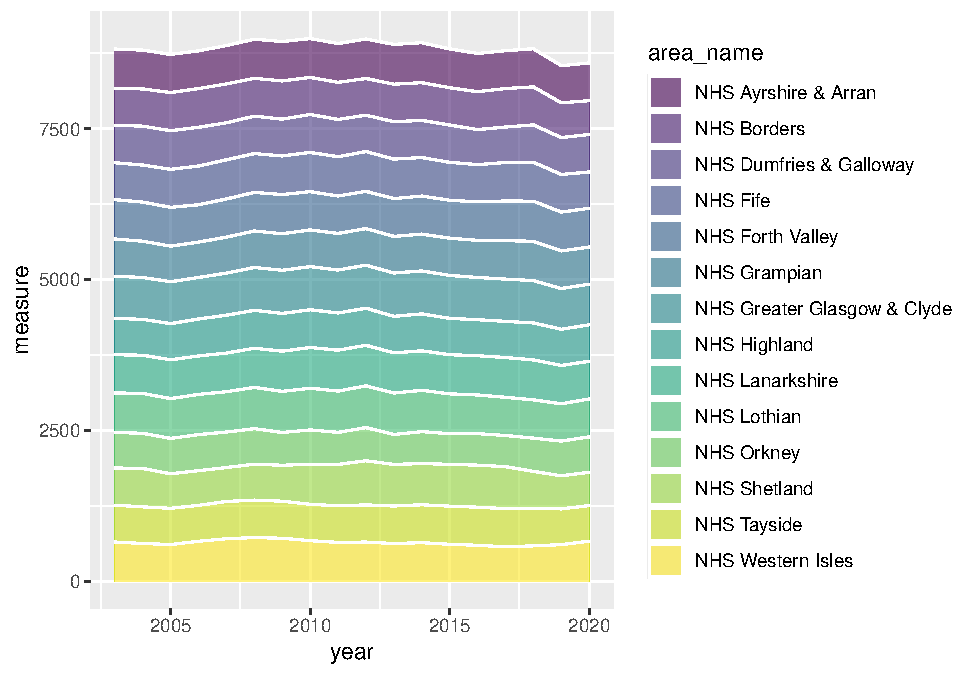
\includegraphics[keepaspectratio]{reportReg_files/figure-latex/unnamed-chunk-4-1.pdf}}

\begin{Shaded}
\begin{Highlighting}[]
\FunctionTok{colorRampPalette}\NormalTok{(}\FunctionTok{c}\NormalTok{(}\FunctionTok{rgb}\NormalTok{(}\DecValTok{1}\NormalTok{,}\DecValTok{0}\NormalTok{,}\DecValTok{0}\NormalTok{,}\DecValTok{0}\NormalTok{), }\FunctionTok{rgb}\NormalTok{(}\DecValTok{0}\NormalTok{,}\DecValTok{0}\NormalTok{,}\DecValTok{1}\NormalTok{,}\DecValTok{0}\NormalTok{)), }\AttributeTok{alpha =} \ConstantTok{TRUE}\NormalTok{)(}\DecValTok{8}\NormalTok{)}
\end{Highlighting}
\end{Shaded}

\begin{verbatim}
## [1] "#FF000000" "#DA002400" "#B6004800" "#91006D00" "#6D009100" "#4800B600"
## [7] "#2400DA00" "#0000FF00"
\end{verbatim}

\begin{Shaded}
\begin{Highlighting}[]
\NormalTok{diffOverYears }\OtherTok{\textless{}{-}} \ControlFlowTok{function}\NormalTok{(year1, year2)\{}
\NormalTok{    result }\OtherTok{=}\NormalTok{ year1 }\SpecialCharTok{{-}}\NormalTok{ year2}
    \ControlFlowTok{if}\NormalTok{ (result }\SpecialCharTok{\textgreater{}=}\DecValTok{0} \SpecialCharTok{\&}\NormalTok{ result}\SpecialCharTok{\textless{}=}\DecValTok{50}\NormalTok{)\{}
\NormalTok{        result }\OtherTok{=} \StringTok{"white"}
\NormalTok{        intensity }\OtherTok{\textless{}{-}} \FunctionTok{max}\NormalTok{(}\DecValTok{0}\NormalTok{, }\FunctionTok{min}\NormalTok{(}\DecValTok{255}\NormalTok{, }\SpecialCharTok{{-}}\NormalTok{value }\SpecialCharTok{*} \DecValTok{51}\NormalTok{))}
        \FunctionTok{rgb}\NormalTok{(}\FunctionTok{colorRampPalette}\NormalTok{(intensity) }\SpecialCharTok{/} \DecValTok{255}\NormalTok{, }\AttributeTok{maxColorValue =} \DecValTok{255}\NormalTok{)}

\NormalTok{    \}}\ControlFlowTok{else} \ControlFlowTok{if}\NormalTok{ (result}\SpecialCharTok{\textless{}}\DecValTok{0}\NormalTok{)\{}

\NormalTok{    \}}
        
\NormalTok{    \}}
\end{Highlighting}
\end{Shaded}

\newpage
\begin{landscape}
\centering
### Summary Table of Data Within Graph 

``` r
healthBoardData <- cancerReg %>%
    group_by(year) %>%
    mutate(Percent = measure / sum(measure) * 100)
healthBoardData <- cancerReg %>% pivot_wider(names_from = year, values_from = measure)
healthBoardData <- healthBoardData %>%
    mutate(
        Average = rowMeans(select(., `2003`:`2020`), na.rm = TRUE)
    )
kable(healthBoardData, format = "latex", booktabs = TRUE)
```


\begin{tabular}{llrrrrrrrrrrrrrrrrrrrr}
\toprule
area\_code & area\_name & 2003 & 2004 & 2005 & 2006 & 2007 & 2008 & 2009 & 2010 & 2011 & 2012 & 2013 & 2014 & 2015 & 2016 & 2017 & 2018 & 2019 & 2020 & 2021 & Average\\
\midrule
S08000015 & NHS Ayrshire \& Arran & 649.7 & 642.8 & 631.6 & 626.1 & 636.4 & 648.2 & 652.2 & 643.8 & 643.2 & 654.3 & 659.6 & 662.1 & 643.4 & 633.9 & 627.2 & 632.8 & 616.0 & 625.5 & NA & 640.4889\\
S08000016 & NHS Borders & 614.6 & 616.8 & 632.7 & 641.5 & 643.5 & 627.5 & 633.8 & 614.8 & 614.5 & 608.5 & 621.2 & 625.5 & 618.9 & 628.1 & 638.1 & 629.3 & 575.6 & 560.1 & NA & 619.1667\\
S08000017 & NHS Dumfries \& Galloway & 620.5 & 645.2 & 639.4 & 642.1 & 613.4 & 619.8 & 609.1 & 628.9 & 617.6 & 602.7 & 619.9 & 616.1 & 617.9 & 580.9 & 588.7 & 618.5 & 611.7 & 621.7 & NA & 617.4500\\
S08000019 & NHS Forth Valley & 651.8 & 648.2 & 642.8 & 618.3 & 633.2 & 638.9 & 649.8 & 634.1 & 620.3 & 617.3 & 626.7 & 630.4 & 628.9 & 638.2 & 657.4 & 664.7 & 643.7 & 642.4 & NA & 638.1722\\
S08000020 & NHS Grampian & 617.8 & 601.5 & 589.7 & 586.6 & 595.9 & 605.0 & 605.4 & 608.5 & 606.2 & 606.8 & 607.1 & 610.3 & 617.1 & 614.8 & 637.4 & 651.1 & 623.3 & 614.9 & NA & 611.0778\\
\addlinespace
S08000022 & NHS Highland & 602.9 & 594.5 & 598.9 & 613.3 & 627.4 & 627.6 & 625.8 & 625.4 & 616.8 & 614.3 & 604.8 & 612.2 & 602.4 & 597.5 & 598.8 & 613.4 & 600.8 & 604.9 & NA & 610.0944\\
S08000024 & NHS Lothian & 655.1 & 660.8 & 659.4 & 666.1 & 668.7 & 683.4 & 681.6 & 691.8 & 684.3 & 691.6 & 686.7 & 684.5 & 659.9 & 641.4 & 632.7 & 635.3 & 617.5 & 628.9 & NA & 662.7611\\
S08000025 & NHS Orkney & 589.0 & 582.4 & 587.1 & 598.1 & 587.4 & 589.3 & 543.0 & 569.2 & 531.3 & 549.1 & 496.1 & 529.1 & 508.0 & 521.7 & 516.3 & 550.7 & 575.9 & 586.6 & NA & 556.1278\\
S08000026 & NHS Shetland & 616.0 & 636.7 & 571.8 & 574.3 & 562.6 & 594.9 & 596.0 & 663.4 & 685.6 & 731.7 & 689.3 & 683.1 & 693.4 & 697.4 & 696.2 & 610.8 & 548.4 & 551.9 & NA & 633.5278\\
S08000028 & NHS Western Isles & 652.0 & 628.1 & 610.3 & 664.4 & 707.2 & 726.0 & 715.0 & 674.4 & 646.0 & 651.6 & 626.6 & 641.8 & 614.6 & 598.1 & 573.3 & 588.7 & 609.0 & 665.8 & NA & 644.0500\\
\addlinespace
S08000029 & NHS Fife & 611.4 & 614.0 & 630.7 & 641.7 & 648.9 & 643.9 & 640.4 & 650.0 & 651.3 & 659.4 & 654.5 & 638.3 & 628.3 & 617.1 & 637.5 & 645.9 & 623.1 & 602.0 & NA & 635.4667\\
S08000030 & NHS Tayside & 611.2 & 607.3 & 600.6 & 596.0 & 617.6 & 621.1 & 613.7 & 603.1 & 606.9 & 616.1 & 622.6 & 627.8 & 632.1 & 631.2 & 632.1 & 623.9 & 592.0 & 590.5 & NA & 613.6556\\
S08000031 & NHS Greater Glasgow \& Clyde & 697.3 & 693.9 & 695.0 & 687.6 & 698.1 & 710.9 & 715.4 & 714.4 & 712.3 & 713.3 & 718.2 & 712.0 & 711.5 & 699.3 & 700.2 & 702.0 & 674.8 & 673.5 & NA & 701.6500\\
S08000032 & NHS Lanarkshire & 633.7 & 632.7 & 643.5 & 637.3 & 640.5 & 649.8 & 665.6 & 675.0 & 677.5 & 672.7 & 666.5 & 654.8 & 649.1 & 650.3 & 659.8 & 661.0 & 635.4 & 624.1 & NA & 651.6278\\
\bottomrule
\end{tabular}
\end{landscape}
\newpage

\#Note for next time: what I want to do at this point is to show the
changing colours as a difference change if its only within a small
amount of chaning values then ignore the calues and do not \#colour the
cell, otherwise red fir a rise and green for a fall

\end{document}
